\documentclass[a4paper, 12pt]{article}

% ===== 宏包 =====
\usepackage[UTF8]{ctex}               % 中文支持
\usepackage[T1]{fontenc}              % T1 编码，提供直引号等字形
\usepackage[margin=2.5cm]{geometry}   % 页边距
\usepackage{amsmath, amssymb}         % 数学公式
\usepackage{booktabs}                 % 三线表
\usepackage{graphicx}                 % 插图
\usepackage{xcolor}                   % 颜色（需在 listings 之前）
\usepackage{listings}                 % 代码块
\usepackage{textcomp}                 % 提供直引号等 TS1 符号
\usepackage{upquote}                  % 代码里的单引号排成直引号，而非弯引号
\usepackage{titlesec}                 % 标题样式
\usepackage{fancyhdr}                 % 页眉页脚
\usepackage{hyperref}                 % 超链接（最后加载）

% ===== 配色：蓝白主题 =====
\definecolor{primary}{HTML}{1F5FA8}   % 主蓝
\definecolor{accent}{HTML}{4A90D9}    % 浅蓝
\definecolor{bgblue}{HTML}{F0F6FC}    % 极浅蓝背景

% ===== 标题样式 =====
\titleformat{\section}{\Large\bfseries\color{primary}}{\thesection}{0.8em}{}
\titleformat{\subsection}{\large\bfseries\color{accent}}{\thesubsection}{0.8em}{}

% ===== 页眉页脚 =====
\pagestyle{fancy}
\fancyhf{}
\fancyhead[L]{\small\color{primary}系统开发工具基础 · 第二周实验报告}
\fancyhead[R]{\small\color{primary}陆立庭 · 25120014018}
\fancyfoot[C]{\small\color{primary}\thepage}
\renewcommand{\headrulewidth}{0.6pt}
\renewcommand{\headrule}{\color{accent}\hrule width\headwidth height\headrulewidth}

% ===== 代码块样式 =====
\lstset{
  basicstyle=\ttfamily\small,
  breaklines=true,
  frame=single,
  rulecolor=\color{accent},
  backgroundcolor=\color{bgblue},
  columns=fullflexible,
  upquote=true,
  showstringspaces=false,
  commentstyle=\color{gray},
  keywordstyle=\color{primary},
  stringstyle=\color{teal},
}

% ===== 超链接样式 =====
\hypersetup{
  colorlinks=true,
  linkcolor=primary,
  urlcolor=accent,
  citecolor=primary,
}

\title{\textbf{\color{primary}系统开发工具基础\quad 第二周实验报告}}
\author{陆立庭\ -\ 25120014018}
\date{2026 年 8 月}

\begin{document}

\maketitle
\vspace{-0.5em}
\noindent{\color{primary}\rule{\textwidth}{1pt}}

\begin{abstract}
本报告围绕第二周四个实验题目展开，覆盖进程控制与信号、开发环境与语义重构、调试器定位缺陷、性能测量与优化四大主题。报告按“实验题目分析与知识点总结”“实验遇到的问题与解决方法”“实验总结”“课后巩固”“GitHub 链接与提交记录”五个部分组织。
\end{abstract}

\tableofcontents
\newpage

% ============================================================
\section{实验题目分析与知识点总结}
% ============================================================

\subsection{题目一：控制一个可清理的后台任务}

\textbf{题目分析}：运行一个持续打印数字的 Shell 脚本，完成赋予执行权限、前台启动、输出重定向、挂起、后台继续、发送信号终止，并验证脚本在退出前完成了清理。

\textbf{知识点}：
\begin{itemize}
  \item \texttt{trap '命令' TERM INT}：注册信号处理器，收到信号时先执行收尾再退出，即“可清理”；
  \item 信号类型：\texttt{SIGTERM}(15) 可捕获、\texttt{SIGKILL}(9) 不可捕获、\texttt{SIGINT}(2)=Ctrl+C、\texttt{SIGTSTP}=Ctrl+Z；
  \item 任务状态机：前台 $\rightarrow$ Ctrl+Z 挂起 $\rightarrow$ \texttt{bg} 后台 $\rightarrow$ \texttt{kill -TERM} 结束；
  \item \texttt{> stdout.log} 与 \texttt{2> stderr.log} 分别记录标准输出、标准错误；\texttt{jobs -p} 动态取得 PID。
\end{itemize}

脚本与关键操作如下：

\begin{lstlisting}[language=bash]
#!/usr/bin/env bash
trap 'echo CLEAN_EXIT >> cleanup.log; exit 0' TERM INT
n=0
while true; do
  echo "$n"
  n=$((n+1))
  sleep 1
done
\end{lstlisting}

\begin{lstlisting}[language=bash]
chmod +x worker.sh
./worker.sh > stdout.log 2> stderr.log   # 前台启动，输出/错误分离
# Ctrl+Z 挂起 → [1]+ Stopped
bg                                        # 后台继续
jobs                                      # [1]+ Running
kill -TERM $(jobs -p)                     # 发送 SIGTERM（不用 kill -9）
jobs                                      # [1]+ Done
cat cleanup.log                           # 输出 CLEAN_EXIT
\end{lstlisting}

\subsection{题目二：语义重构与本地开发反馈}

\textbf{题目分析}：在已配置 Python 语言服务器的编辑器中，对一个跨文件的函数名完成“跳转到定义、查找引用、重命名符号”，再用 \texttt{ruff} 做静态检查、\texttt{pytest} 跑测试，保证重构不破坏行为。

\textbf{知识点}：
\begin{itemize}
  \item 语言服务器（LSP）：解析整个项目建立符号表，支撑跳转/引用/重命名；
  \item \texttt{F12} 跳转到定义、\texttt{Shift+F12} 查找引用、\texttt{F2} 语义重命名（只改符号、同步所有引用，注释中的同名文字不变）；
  \item \texttt{ruff} 静态检查：不运行代码即可发现“未使用导入”（规则 \texttt{F401}）；
  \item \texttt{pytest}：\texttt{test\_} 开头的函数自动被发现，\texttt{assert} 断言。
\end{itemize}

三个源文件与检查流程：

\begin{lstlisting}[language=python]
# math_utils.py
def total_price(price: float, count: int) -> float:
    return price * count

# app.py
from math_utils import total_price
print(total_price(12.5, 4))

# test_math_utils.py
from math_utils import total_price
def test_total_price():
    assert total_price(12.5, 4) == 50.0
\end{lstlisting}

\begin{lstlisting}[language=bash]
# 在 app.py 临时加入 import os 制造未使用导入
ruff check app.py          # 报 F401 'os' imported but unused
# 删除 import os 后
ruff check .               # All checks passed!
pytest                     # 1 passed
\end{lstlisting}

重命名符号 \texttt{total\_price} $\rightarrow$ \texttt{calculate\_total}，三处引用同步改变。

\subsection{题目三：用调试器定位归并排序缺陷}

\textbf{题目分析}：归并排序的 \texttt{merge} 函数存在一处下标错误，先用调试器定位，再最小修复，最后补回归测试。

\textbf{知识点}：
\begin{itemize}
  \item 调试五步：复现 $\rightarrow$ 断点 $\rightarrow$ 观察变量 $\rightarrow$ 定位 $\rightarrow$ 最小修复 $\rightarrow$ 回归测试；
  \item 归并排序：分治，递归拆到单个元素再两两合并有序数组；
  \item \texttt{merge} 核心：双游标 $i$（左）、$j$（右），每次取两数组头部较小者；
  \item 缺陷本质：右数组该用右游标 \texttt{j}，代码写成 \texttt{right[i]}（用左游标取右数组）。
\end{itemize}

缺陷代码与调试：

\begin{lstlisting}[language=python]
def merge(left, right):
    result = []
    i = j = 0
    while i < len(left) and j < len(right):
        if left[i] <= right[j]:
            result.append(left[i]); i += 1
        else:
            result.append(right[i]); j += 1   # 缺陷：应为 right[j]
    return result + left[i:] + right[j:]
\end{lstlisting}

\begin{lstlisting}[language=bash]
python merge_sort.py        # 输出错误排序结果，复现 bug
python -m pdb merge_sort.py # 进入调试器
# (Pdb) break merge_sort.py:7   ← while 循环行设断点
# (Pdb) continue
# (Pdb) p i                     ← 对比 i、j 发现错位
# (Pdb) p j
\end{lstlisting}

最小修复 \texttt{right[i]} $\rightarrow$ \texttt{right[j]}（仅改一个字符），并补两个测试：

\begin{lstlisting}[language=python]
# test_merge_sort.py
from merge_sort import merge_sort
def test_given():
    assert merge_sort([3,1,4,1,5,9,2,6]) == [1,1,2,3,4,5,6,9]
def test_duplicates():
    assert merge_sort([2,2,1,2,1]) == [1,1,2,2,2]
\end{lstlisting}

\subsection{题目四：先测量，再优化慢速词频程序}

\textbf{题目分析}：先用 \texttt{time} 计时、\texttt{cProfile} 定位热点，再把列表去重优化为 \texttt{set}，在不改变最终 \texttt{count} 的前提下计算加速比。

\textbf{知识点}：
\begin{itemize}
  \item \texttt{time} 测总耗时（跑 2 次取中位数），\texttt{cProfile -s cumulative} 定位耗时热点；
  \item 列表 \texttt{in} 是线性扫描 $O(n)$，\texttt{set} 是哈希查找 $O(1)$，整体 $O(n^2)\rightarrow O(n)$；
  \item 优化原则：行为不变（\texttt{count} 一致）、不写死答案；
  \item 加速比 = 优化前中位数 $\div$ 优化后中位数。
\end{itemize}

测量与优化：

\begin{lstlisting}[language=python]
# 优化前：列表 in 线性扫描 O(n^2)
words = open("words.txt", encoding="utf-8").read().split()
unique = []
for word in words:
    if word not in unique:
        unique.append(word)
print("count=", len(unique))

# 优化后：set 哈希查找 O(n)
words = open("words.txt", encoding="utf-8").read().split()
unique = set(words)
print("count=", len(unique))
\end{lstlisting}

\begin{lstlisting}[language=bash]
time python wordfreq.py      # 跑 2 次取中位数
python -m cProfile -s cumulative wordfreq.py
# 热点：if word not in unique（列表线性查找）
\end{lstlisting}

实测结果见表~\ref{tab:perf}：

\begin{table}[h]
  \centering
  \begin{tabular}{ccc}
    \toprule
    \textbf{版本} & \textbf{中位数耗时} & \textbf{count} \\
    \midrule
    优化前（列表） & 0.160 s & 1000 \\
    优化后（set）  & 0.088 s & 1000 \\
    \bottomrule
  \end{tabular}
  \caption{第8题优化前后对比}
  \label{tab:perf}
\end{table}

加速比 $= 0.160 \div 0.088 \approx 1.8$ 倍。数据集为 30000 词、1000 个唯一词，列表线性查找未出现最坏情况，故加速比有限；在更大词表下 $O(n^2)$ 与 $O(n)$ 的差距会急剧放大。

% ============================================================
\section{实验遇到的问题与解决方法}
% ============================================================

\subsection{问题一：终端选错，time 命令失效}

\textbf{问题描述}：在 VS Code 里运行 Python 计时命令时误用了 \texttt{cmd} 终端，其 \texttt{time} 是“查看/设置系统时间”，并非计时工具，导致命令报错、无法计时。

\textbf{解决方法}：改用 \textbf{Git Bash} 终端（提示符为 \texttt{MINGW64}、结尾 \texttt{\$}），其中 \texttt{time} 才是 bash 的计时关键字。此后所有 Shell 命令统一在 Git Bash 里执行。

\subsection{问题二：pdb 断点设置不熟练}

\textbf{问题描述}：初次使用调试器，不知道如何设置断点、单步执行、查看变量，进入 pdb 后不知下一步该做什么。

\textbf{解决方法}：掌握 pdb 基本命令——\texttt{break 行号} 设断点、\texttt{continue} 运行到断点、\texttt{p 变量名} 打印变量、\texttt{n} 单步、\texttt{q} 退出。在 \texttt{merge} 函数的 while 循环处设断点，对比 \texttt{i}、\texttt{j} 的值定位缺陷。

\subsection{问题三：ruff check 输出看不懂}

\textbf{问题描述}：运行 \texttt{ruff check} 后，对输出信息（如 \texttt{F401 'os' imported but unused}）的含义不理解。

\textbf{解决方法}：明白 ruff 是静态检查器，输出格式为“规则编号 + 说明”。\texttt{F401} 表示“导入了但未使用”，据此删掉无用的 \texttt{import os} 即可通过检查。

\subsection{问题四：优化后反而用时更长}

\textbf{问题描述}：把列表去重改成 \texttt{set} 后，用 \texttt{time} 计时发现优化后反而更慢，一度怀疑优化方向错误。

\textbf{解决方法}：多次计时取中位数后发现，二者耗时都在百毫秒量级，受系统负载影响波动大，单次对比不可靠；且词表去重后仅 1000 个唯一词，列表线性查找未出现最坏情况，加速比本就不大。最终取中位数对比：0.160 s $\rightarrow$ 0.088 s，加速比约 1.8 倍，优化确实有效。

% ============================================================
\section{实验总结}
% ============================================================

通过本周实验，我系统地掌握了以下内容：

\begin{itemize}
  \item \textbf{F2 / F12 的运用}：掌握语言服务器的“跳转到定义、查找引用、语义重命名”，体会到 F2 重命名比全局替换更安全；
  \item \textbf{递归代码运行顺序}：通过给递归函数加打印，看清了“先深入、后返回”的两阶段执行过程；
  \item \textbf{代码效率计时}：学会用 \texttt{time} 测耗时、用 \texttt{cProfile} 找热点，理解列表与 \texttt{set} 的复杂度差异；
  \item \textbf{jobs 任务运行状态}：熟悉前台/后台切换、\texttt{jobs}/\texttt{bg}/\texttt{fg} 查看与控制任务，以及 \texttt{trap} 实现优雅退出。
\end{itemize}

进程控制、重构、调试与性能分析是工程开发中的高频技能。本周的实验让我体会到：性能优化必须“先测量、后动手”，调试必须先复现、再定位，这些方法意识比具体命令更值得长期保留。

% ============================================================
\section{课后巩固：12 个实例练习}
% ============================================================

为巩固本周四道题的知识点，我课后额外做了 12 个由浅入深的实例练习，覆盖进程控制、开发环境、调试、性能优化四个方向，每个实例都按照“练什么 → 任务 → 思路 → 参考 → 自查”的流程完成。下表是这 12 个实例的总览：

\begin{table}[h]
  \centering
  \small
  \begin{tabular}{cllp{6.5cm}}
    \toprule
    \textbf{\#} & \textbf{实例} & \textbf{主题} & \textbf{覆盖知识点} \\
    \midrule
    1 & 前后台初体验 & 进程控制 & \texttt{\&}、\texttt{jobs}、\texttt{fg}、Ctrl+Z、\texttt{bg} \\
    2 & 输出与错误分开 & 进程控制 & \texttt{>} 与 \texttt{2>} 重定向分离 \\
    3 & trap 捕获信号 & 进程控制 & \texttt{trap}、\texttt{kill -TERM} vs \texttt{-9} \\
    4 & F12 跳转定义 & 开发环境 & LSP 跳转到定义 \\
    5 & F2 语义重命名 & 开发环境 & 语义重命名（符号≠文字） \\
    6 & ruff 抓未用导入 + pytest & 开发环境 & \texttt{F401} 静态检查、写测试 \\
    7 & pdb 入门 & 调试 & 断点、单步、\texttt{p} 打印变量 \\
    8 & 递归与归并理解 & 调试 & 递归过程可视化 \\
    9 & 调试一个排序 bug & 调试 & 定位修复 + 回归测试 \\
    10 & time 计时对比 & 性能优化 & \texttt{time} 测耗时、对比实现 \\
    11 & cProfile 找热点 & 性能优化 & 定位耗时集中处 \\
    12 & 复杂度对比 + set 优化 & 性能优化 & \texttt{list} vs \texttt{set}、$O(n^2)\rightarrow O(n)$ \\
    \bottomrule
  \end{tabular}
  \caption{课后巩固的 12 个实例总览}
  \label{tab:practice2}
\end{table}

\subsection{解题感悟}

课后我按这 12 个实例把本周的知识点从头到尾敲了一遍。感受最深的是“环境”和“方法”这两件事。前者是教训：一开始在 cmd 里敲 \texttt{time} 怎么都报错，折腾半天才发现该用 Git Bash——工具选错，再努力也白搭。后者是体会：调试那几道题，光看别人说“指针错位”完全没感觉，非得自己 \texttt{break} 下去、\texttt{p} 一下变量，盯着 \texttt{i} 和 \texttt{j} 的值，才突然看明白 bug 到底在哪。性能优化也一样，列表换成 \texttt{set} 就一行代码，但如果不是先 \texttt{time}、再 \texttt{cProfile} 一步步测下来，我根本不会知道“慢”到底慢在哪一行。这些工具不亲手上手敲，道理永远停在纸上。

完整版（含每个实例的思路与参考代码）已随仓库上传，可在 GitHub 仓库的 \href{https://github.com/lyun69965/primary-system-tools}{\texttt{第2周\_12个实例练习.md}} 中阅读和复制代码。

% ============================================================
\section{附录：GitHub 链接与提交记录}
% ============================================================

本次实验代码已提交至 GitHub 仓库，地址如下：

\begin{center}
  \url{https://github.com/lyun69965/primary-system-tools.git}
\end{center}

下图为本仓库的 commit 提交记录截图：

\begin{figure}[h]
  \centering
  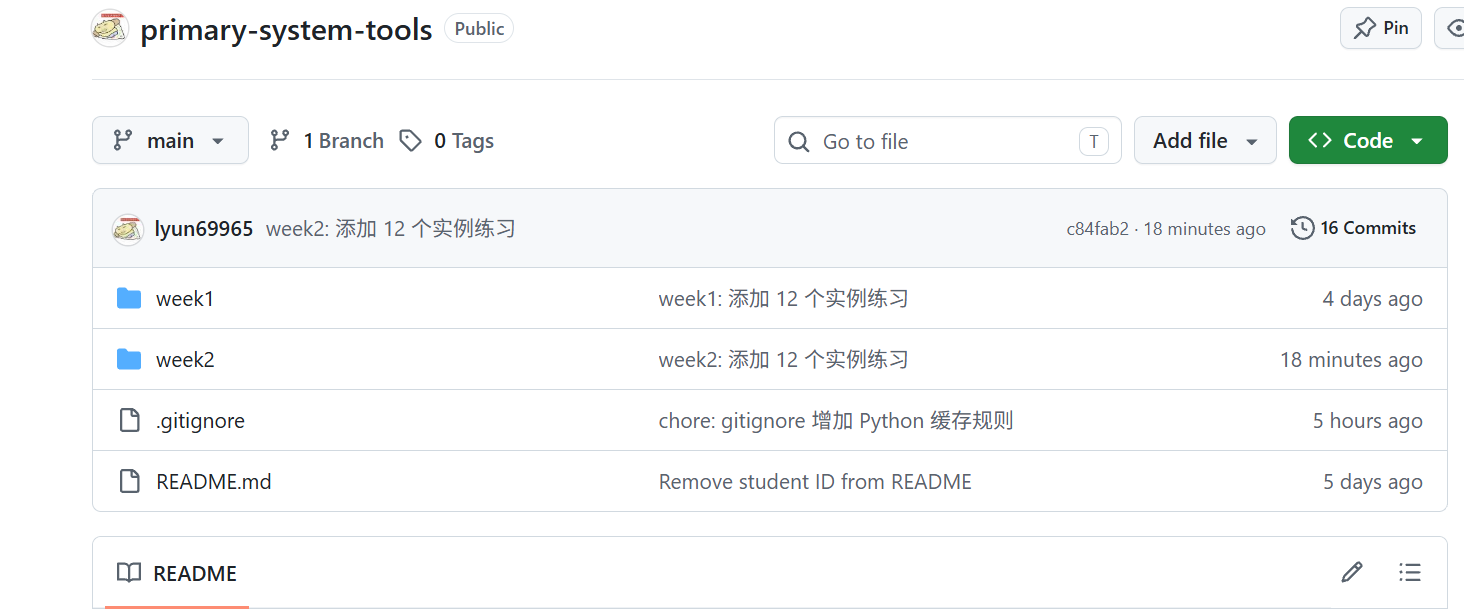
\includegraphics[width=0.85\textwidth]{commit_week2.png}
  \caption{GitHub 仓库 commit 提交记录}
  \label{fig:commit2}
\end{figure}

\end{document}
